\section{Software}

\begin{frame}
  \tableofcontents[currentsection,hideothersubsections]
\end{frame}


\begin{frame}
  \frametitle{Wire Cell Software Ecosystem}

  Wire Cell breaks up into three main parts:

  \begin{description}
  \item[visualization] the ``Bee'' web application (Chao Zhang)
  \item[prototype] reconstruction algorithms, initial proof of
    principle (Xin Qian)
  \item[toolkit] production process, parallelism and for long-term development (bv)
  \end{description}

\end{frame}

\subsection{Bee Display}

\begin{frame}
  \frametitle{Bee: an interactive 3D visualization system}

  Select features:
  \begin{itemize}
  \item Browser-based, general purpose 3D event display, 
  \item Implemented in \textbf{JavaScript/WebGL} + \textbf{Django}.
  \item Displays reconstructed and ``true'' information.
  \item Simple \textbf{JSON} data file format, 
    \begin{itemize}
    \item \href{http://bnlif.github.io/wire-cell-docs/viz/uploads/}{drag-and-drop user
      file uploads}.
    \end{itemize}
  \item \textbf{Bee 2.0} will add interactive human-guided
    reconstruction at the pattern recognition level.
  \end{itemize}
\end{frame}

\begin{frame}
  \frametitle{Interactive 3D visualization}
  \begin{center}
    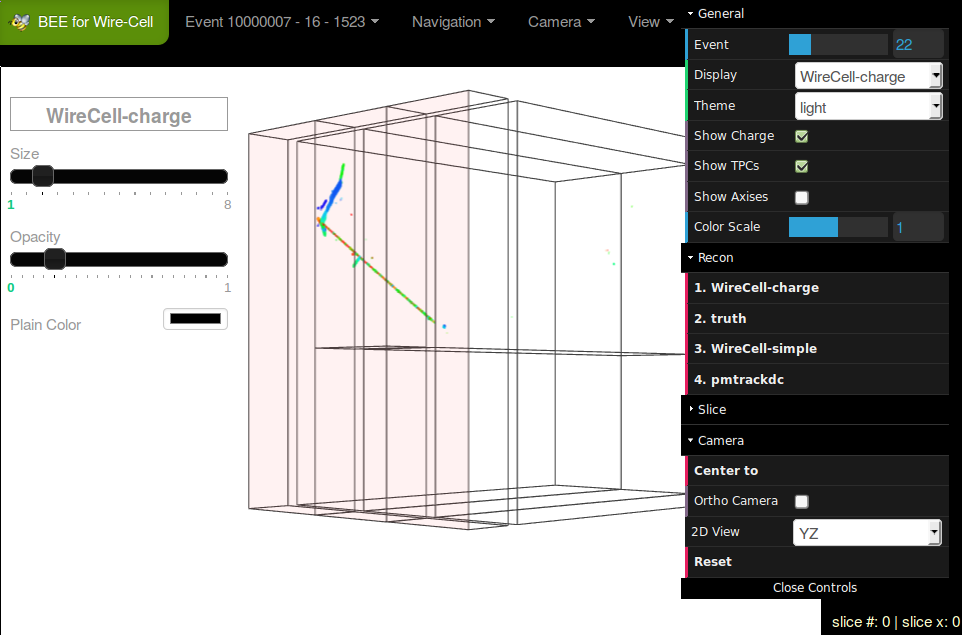
\includegraphics[height=0.7\textheight]{bee-full-gui.png}    
  \end{center}
  \begin{center}
    Try it yourself: \url{http://www.phy.bnl.gov/wire-cell/bee/}
  \end{center}
\end{frame}


\subsection{Prototype}

\begin{frame}
  \frametitle{Wire Cell Working Prototype}
  \footnotesize

  \begin{itemize}
  \item \textbf{Very successful proof of principle!}
  \item Currently \textbf{leads the state of the art} in LArTPC
    reconstruction techniques.
  \item Amazingly fast development (\textbf{Xin Qian}!)
  \end{itemize}

  \begin{center}
    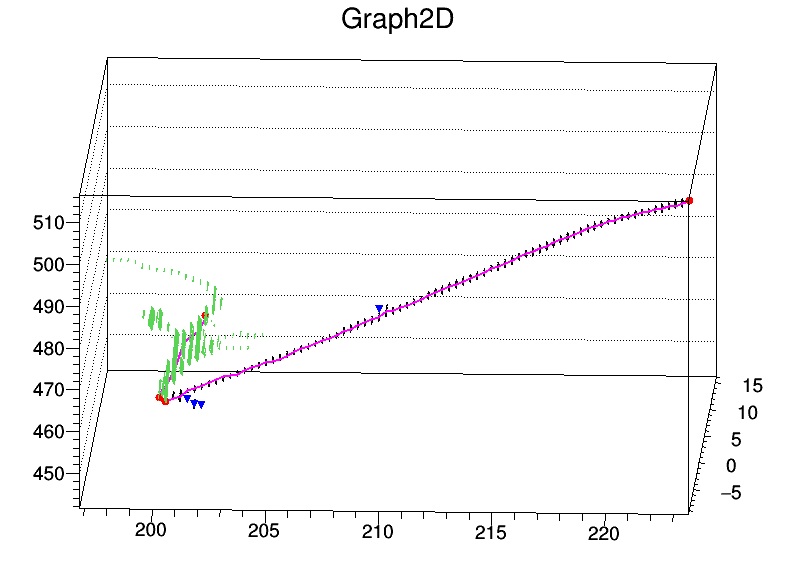
\includegraphics[height=0.5\textheight,trim=0cm 0cm 0cm 2cm,clip]{xin-shower.png}

    \scriptsize
    Colors indicate identified tracks and showers.
  \end{center}

\end{frame}

\subsection{Toolkit}

\begin{frame}
  \frametitle{Wire Cell Toolkit}

  \begin{columns}
    \begin{column}{0.65\paperwidth}
    \end{column}
    \begin{column}{0.35\paperwidth}
      \vspace{-20mm}
      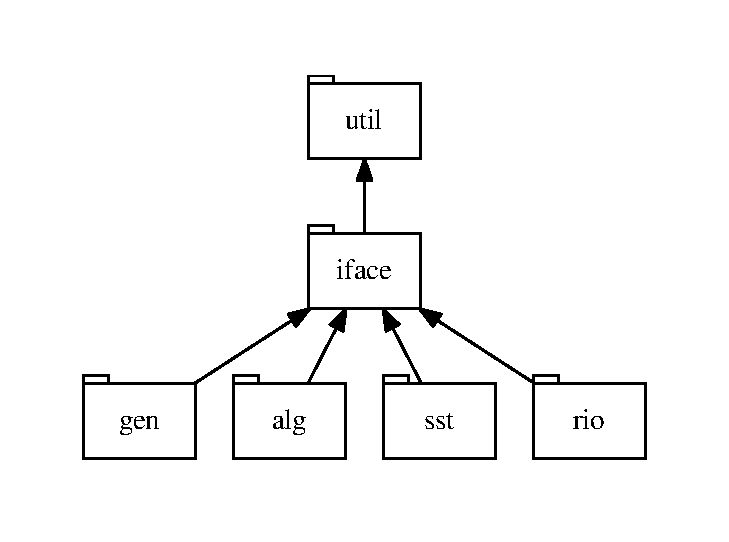
\includegraphics[width=\textwidth]{deps.pdf}      
    \end{column}
  \end{columns}

  \vspace{-15mm}

  Address compromises made in the name\\
  of rapid prototyping 
  \begin{itemize}
  \item Includes \textbf{packaging and build} system.
  \item Comprehensive \textbf{API} via abstract interface classes.
  \item Mindful of \textbf{dependencies}, external and internal.
  \item Built-in wire and cell \textbf{geometry descriptions} or load from file.
  \item Includes simple \textbf{LArTPC detector simulation}.
  \item Rewriten implementations of core \textbf{prototype algorithms}.
  \item Abstracted \textbf{Data Flow Programming execution model}
  \end{itemize}

  \vfill

  Just now becoming available, but more work to do.

\end{frame}

\begin{frame}[fragile]
  \frametitle{Wire Cell Execution Model}

  \begin{columns}
    \begin{column}{0.7\textwidth}
      \footnotesize 
      The toolkit supports \textbf{data flow programming} paradigm
      \begin{itemize}
        \item Design influenced by
          \href{http://www0.bnl.gov/events/details.php?q=8932}{VisTrails} and others.
        \item Data flows through a graph made from:
          \begin{description}
          \item[vertices:] computational units / algorithms
          \item[edges:] data queues of a given type
          \end{description}
        \item Streamed processing minimizes RAM usage.
        \item High-level ``graph programming'' in user config.
        \item \textbf{Thread-safe queues $\Rightarrow$ parallel processing.}
        \item Abstract graph execution machinery.
          \begin{itemize}\scriptsize
          \item Intel TBB provides reference implementation.
          \end{itemize}
        \item Encourages isolated, targeted development and testing of each
          compute vertex.
        \item Feedback loops to implement iterative workflows.
        \end{itemize}
      \end{column}
      \begin{column}{0.3\textwidth}

        \vspace{-10mm}

        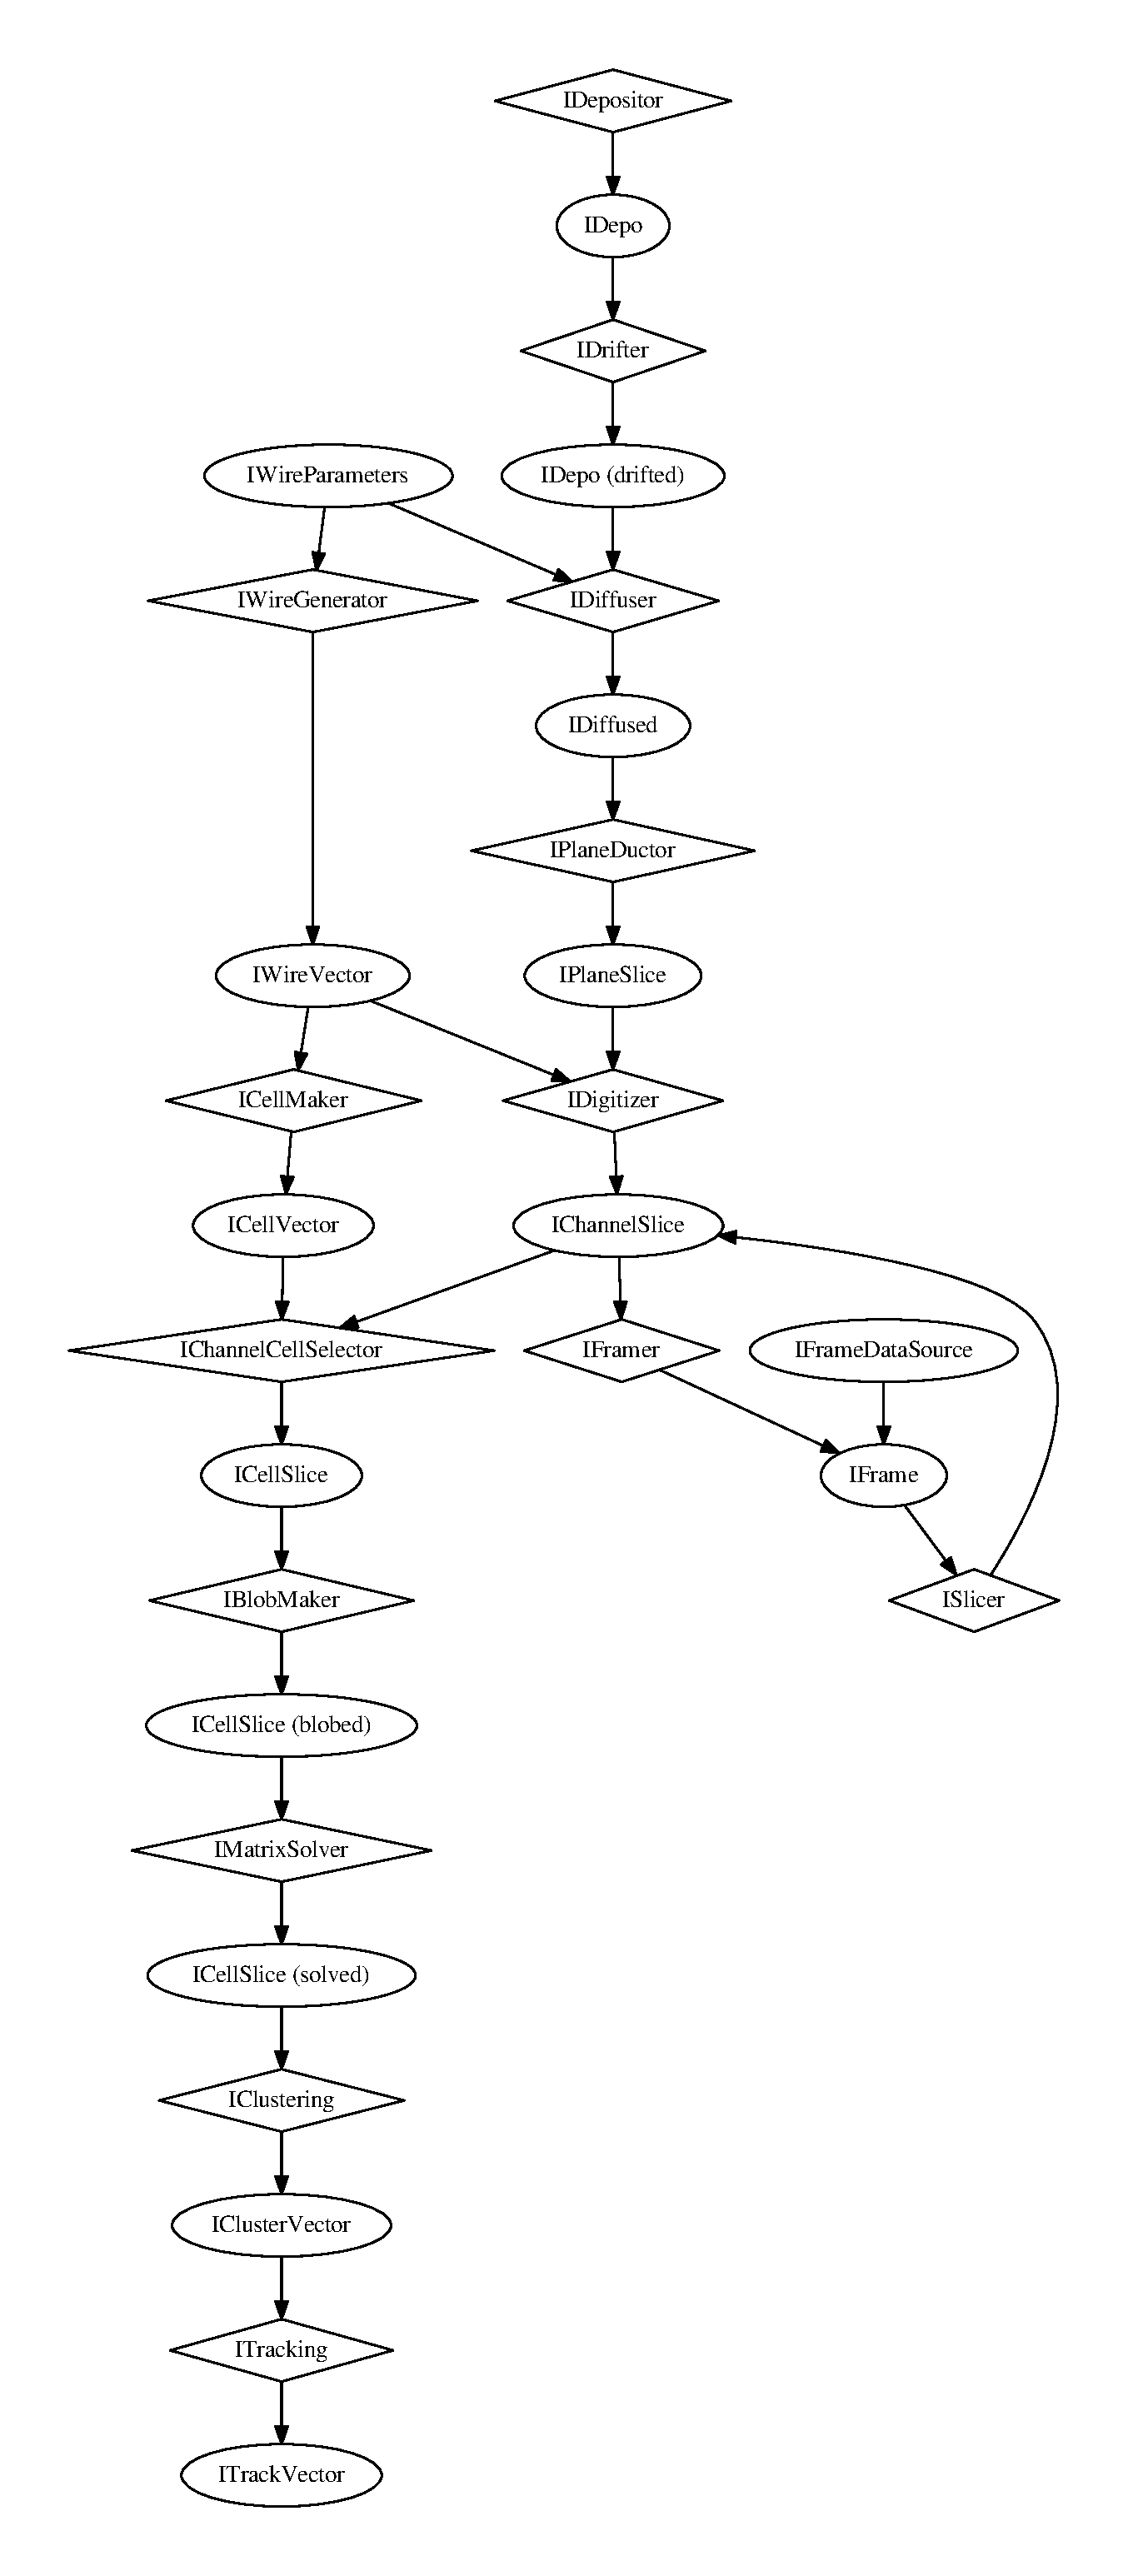
\includegraphics[width=\textwidth]{dataflow.pdf}

        \tiny One possible high-level flow.
      \end{column}
    \end{columns}
\end{frame}

